\documentclass[12pt]{article}%
\usepackage{amsfonts}
\usepackage{fancyhdr}
\usepackage{comment}
\usepackage[a4paper, top=2.5cm, bottom=2.5cm, left=2.2cm, right=2.2cm]%
{geometry}
\usepackage{times}
\usepackage{amsmath}
\usepackage{changepage}
\usepackage{amssymb}
\usepackage{graphicx}%
\setcounter{MaxMatrixCols}{30}
\newtheorem{theorem}{Theorem}
\newtheorem{acknowledgement}[theorem]{Acknowledgement}
\newtheorem{algorithm}[theorem]{Algorithm}
\newtheorem{axiom}{Axiom}
\newtheorem{case}[theorem]{Case}
\newtheorem{claim}[theorem]{Claim}
\newtheorem{conclusion}[theorem]{Conclusion}
\newtheorem{condition}[theorem]{Condition}
\newtheorem{conjecture}[theorem]{Conjecture}
\newtheorem{corollary}[theorem]{Corollary}
\newtheorem{criterion}[theorem]{Criterion}
\newtheorem{definition}[theorem]{Definition}
\newtheorem{example}[theorem]{Example}
\newtheorem{exercise}[theorem]{Exercise}
\newtheorem{lemma}[theorem]{Lemma}
\newtheorem{notation}[theorem]{Notation}
\newtheorem{problem}[theorem]{Problem}
\newtheorem{proposition}[theorem]{Proposition}
\newtheorem{remark}[theorem]{Remark}
\newtheorem{solution}[theorem]{Solution}
\newtheorem{summary}[theorem]{Summary}
\newenvironment{proof}[1][Proof]{\textbf{#1.} }{\ \rule{0.5em}{0.5em}}

\newcommand{\Q}{\mathbb{Q}}
\newcommand{\R}{\mathbb{R}}
\newcommand{\C}{\mathbb{C}}
\newcommand{\Z}{\mathbb{Z}}

\begin{document}

\title{CS280 Fall 2022 Assignment 3 \\ Part A}
\author{RNN, LSTM and GRU}
\maketitle

\paragraph{Name:Dai ZiJia}

\paragraph{Student ID:2022233158}

\newpage


\subsubsection*{1. Parity-check network (16 points)}
Note that the initial parity bit is 1, what's the relation between each input and the previous parity bit? Determine the relation between the parity and inputs and complete the parity bits($p_1,p_2,p_3,p_4$) and design and draw a RNN to predict parity. 
	
	\begin{align*}
	    \textit{Parity bits}&:\quad\quad0\quad0\quad0\quad1\quad0\quad1\quad p_1\quad p_2\quad p_3 \quad p_4 \quad\rightarrow \\
	    \textit{Input}&:\quad\quad0\quad1\quad1\quad0\quad0\quad0\quad1\qquad1\quad0\qquad0
	\end{align*}

\begin{figure}[!h]
	\centering
	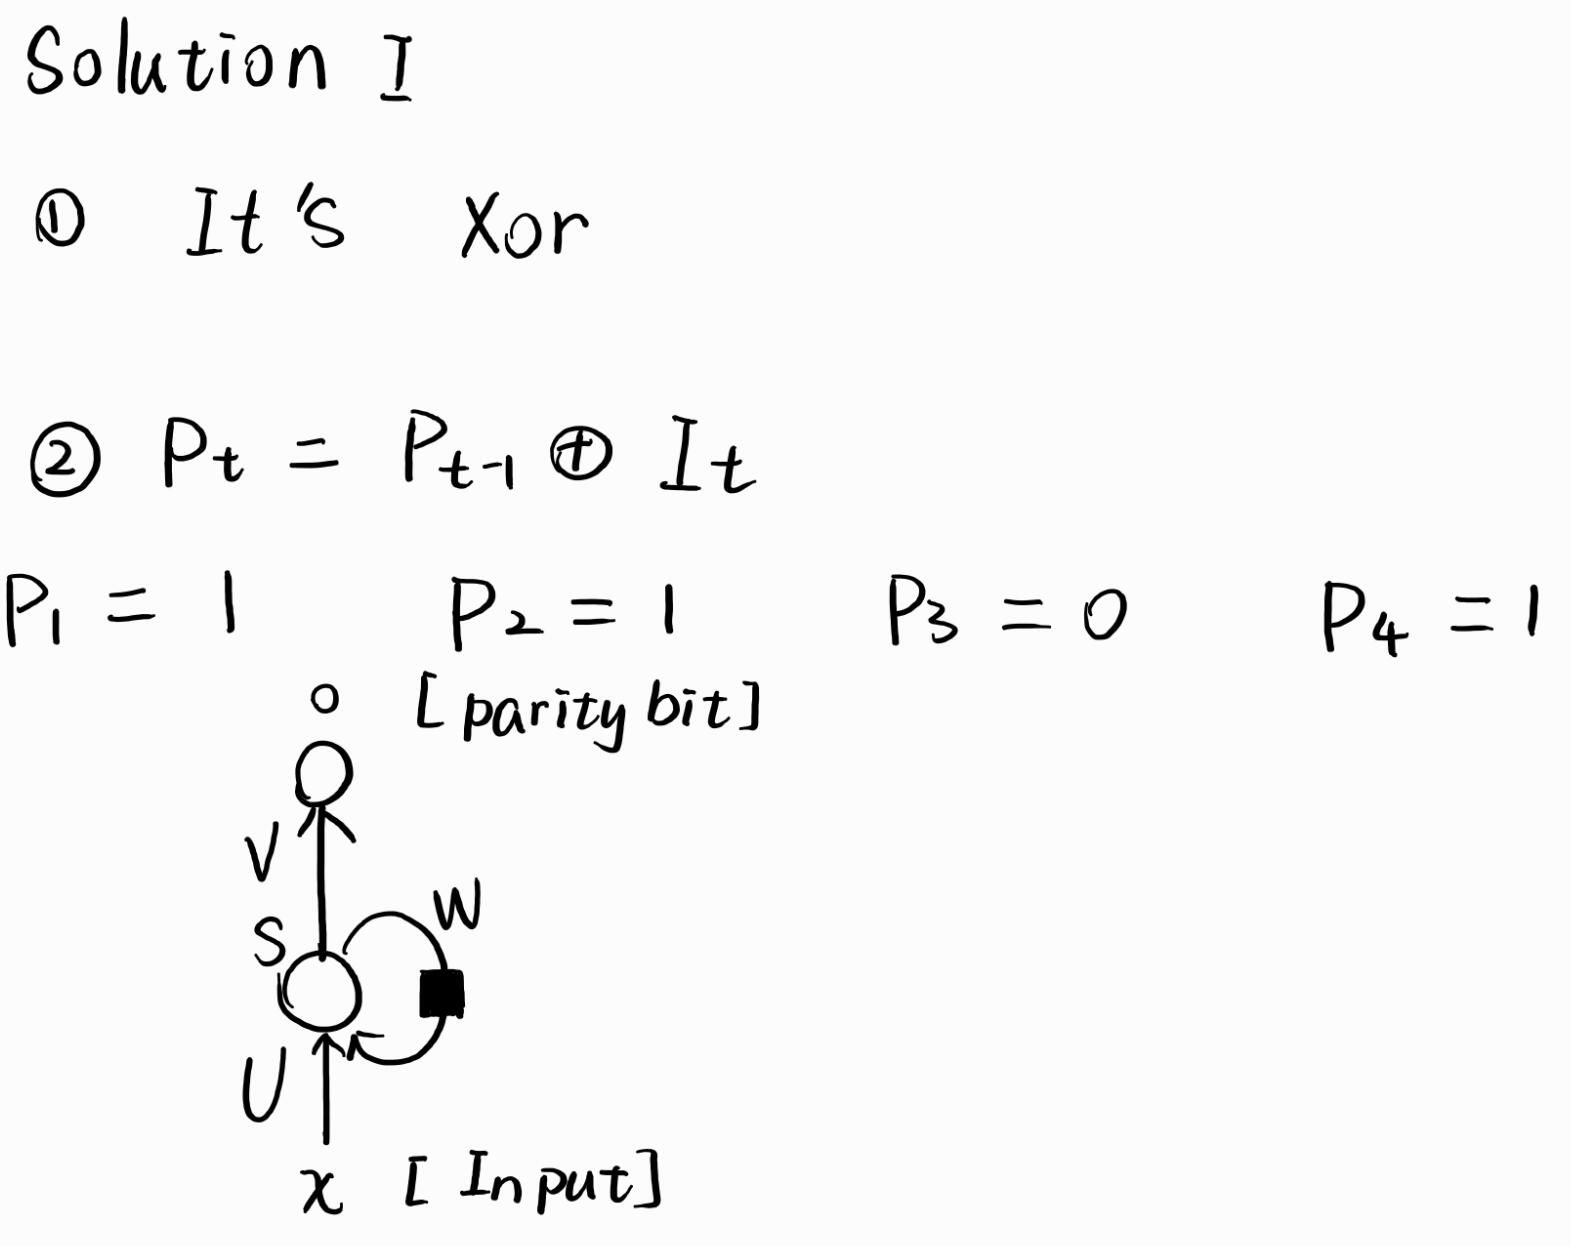
\includegraphics[width=5in]{1.jpg}
\end{figure}

\newpage


\subsubsection*{2. GRU (17 points)}

1. Draw the diagram of GRU, describe the gates (where? What is the role of each gate?), and point out the differences between GRU and LSTM in the design of gates.\\
2. In what situations(s) is LSTM/GRU used respectively? Explain your reason.

\begin{figure}[!h]
	\centering
	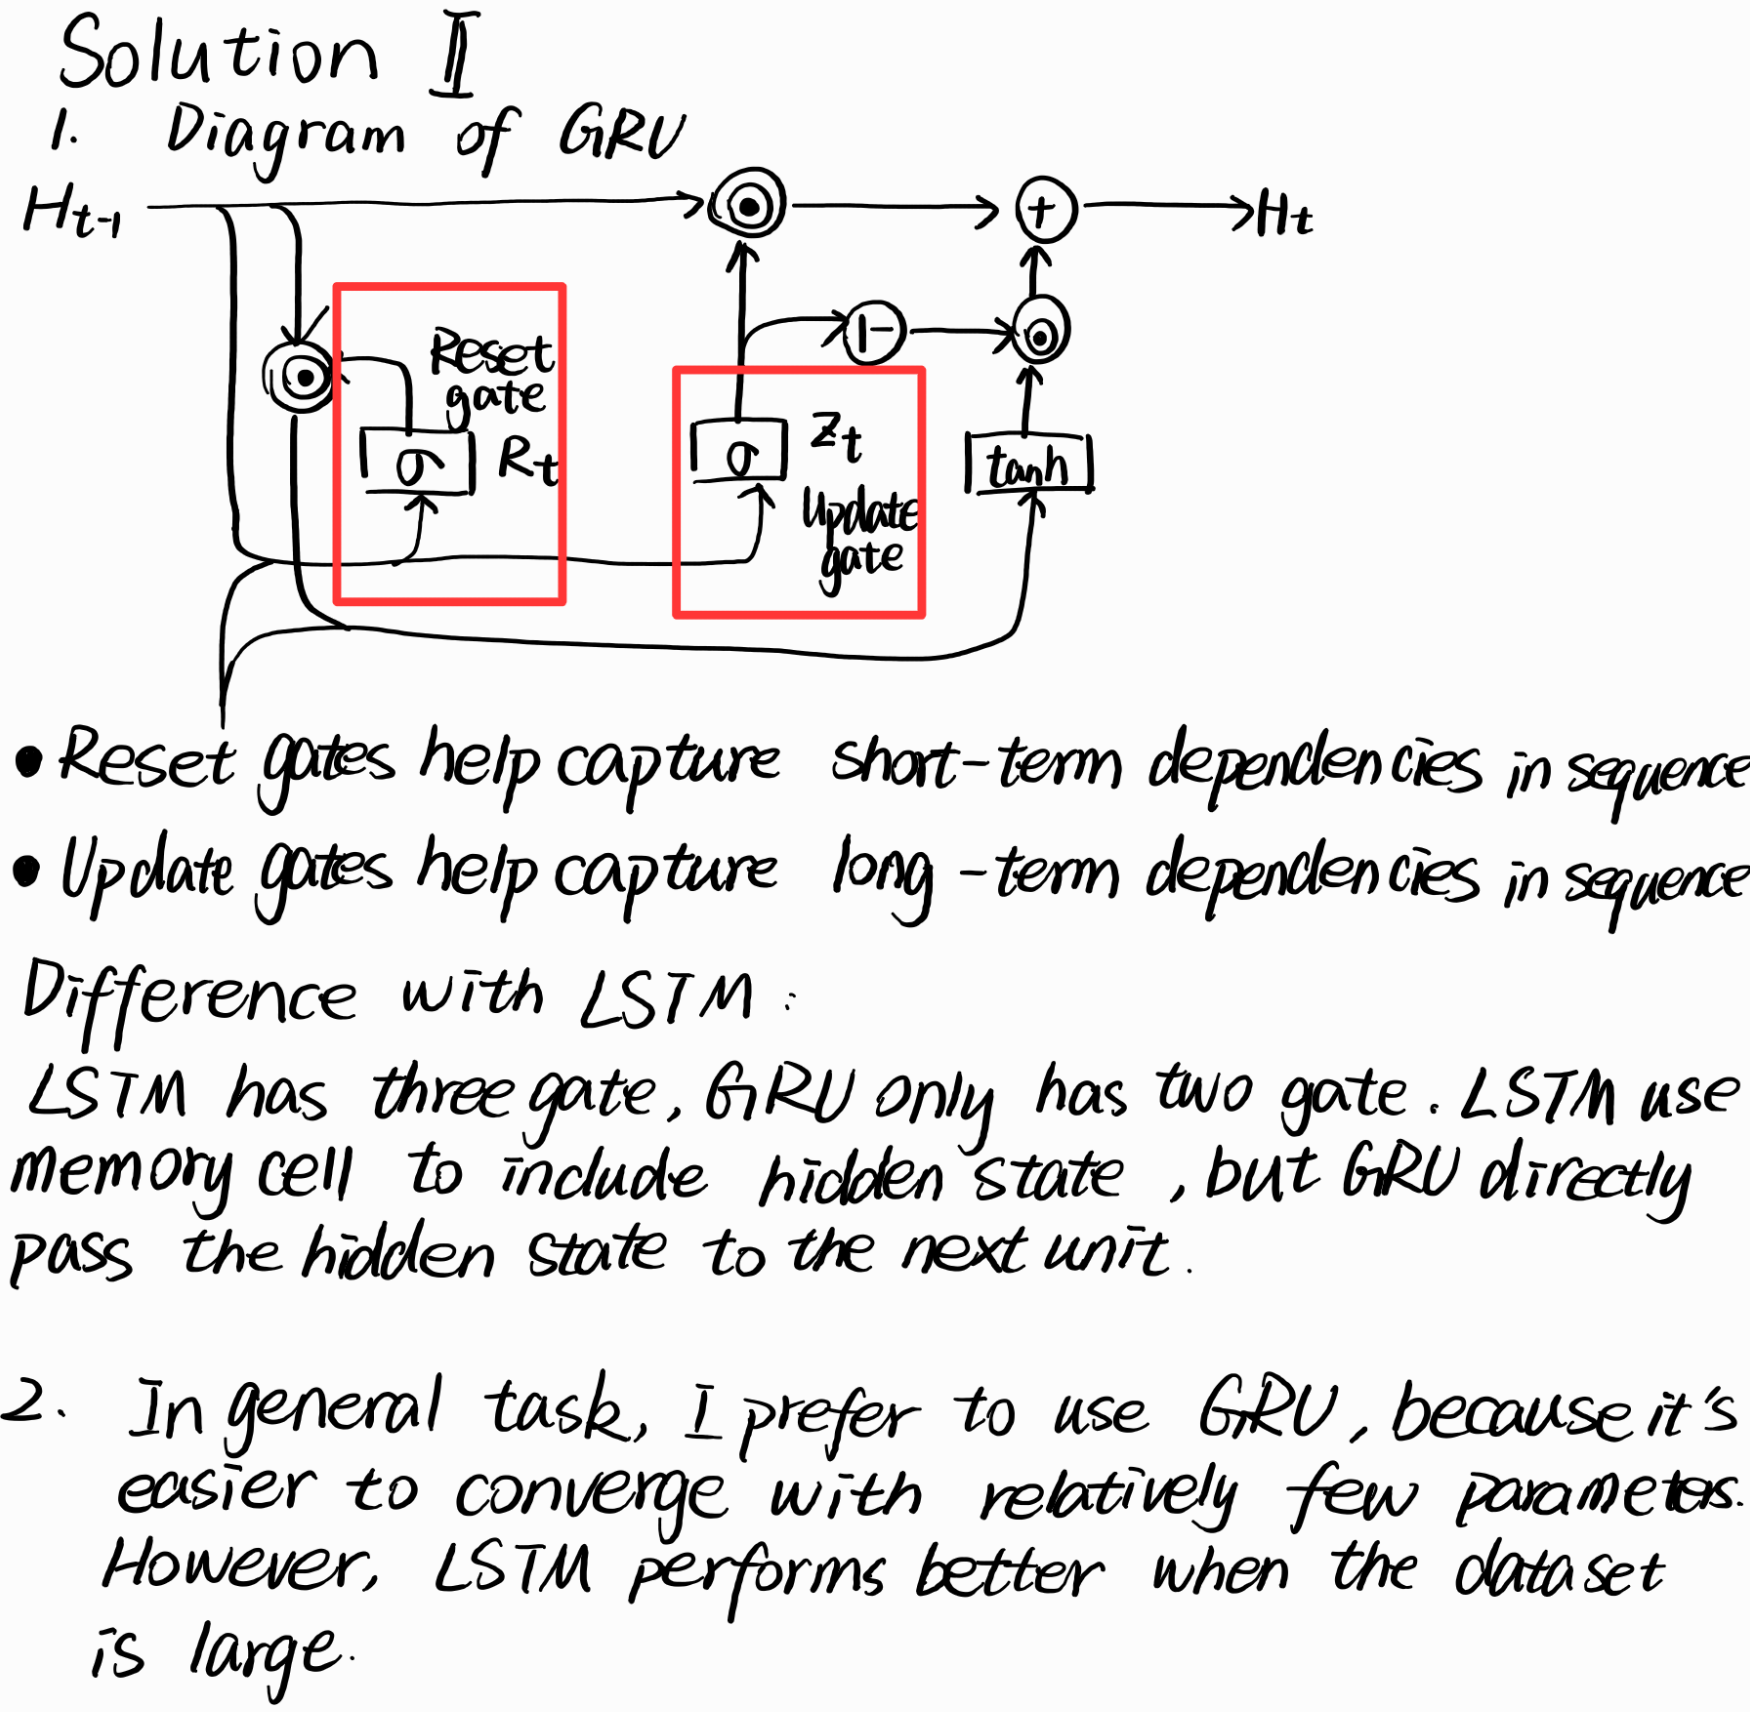
\includegraphics[width=5in]{2.png}
\end{figure}
\newpage





\end{document}